\chapter{Résultats et analyses}
\label{chapitre:resultats}

Ce chapitre présente les preuves techniques du système. La première partie montre la réponse
de la branche HYPO à des dégradations graduelles, son
avantage sur les comparateurs IF/LOF et sa stabilité locale par OFAT. La deuxième partie
teste sa robustesse à des formes moins favorables à aire d'enveloppe appariée, puis examine l'extension
INSTABILITÉ et les règles de fusion sur une campagne plus large. Les
pourcentages décrivent la réponse du logiciel à des scénarios contrôlés et permettent de
comparer la détection, la localisation et la charge de vérification. Le Tableau~\ref{tab:cles_lecture_resultats}
présente les clés de lecture mobilisées tout au long de ce chapitre.

Aucun étalon vétérinaire n'accompagne le corpus principal~: la performance ne se lit donc pas
en valeur absolue. Elle se juge de trois façons. La première est l'écart à l'exécution propre
de la même vache, qui isole ce que l'injection seule produit. La deuxième est la comparaison
aux quatre configurations alternatives appliquées aux mêmes fenêtres, qui situe l'apport de la
structure temporelle et multivariée. La troisième est le respect des conditions de portée
fixées au Chapitre~\ref{chapitre:systeme} avant la campagne, pour la sélection des règles de
fusion. Le Tableau~\ref{tab:objectifs_resultats}, en fin de chapitre, confronte chaque
objectif annoncé à son résultat.

% =====================================================================
\section{Clés de lecture et intégrité des protocoles}
% =====================================================================
\begin{table}[H]
  \centering
  \caption{Clés de lecture du chapitre.}
  \label{tab:cles_lecture_resultats}
  \small
  \begin{tabular}{p{0.28\textwidth}p{0.64\textwidth}}
    \toprule
    Élément & Interprétation \\
    \midrule
    Vaches admissibles
      & Seules onze des 28 vaches possèdent une période future suffisamment longue, les signaux
        requis et une couverture compatible avec toutes les campagnes. \\
    Injections après la période de référence
      & Elles commencent après les 60\,\% réservés à la construction de la référence; les
        données injectées ne peuvent donc pas influencer cette référence. \\
    Attribution
      & Une alerte est attribuable seulement si elle apparaît avec l'injection et non dans
        l'exécution propre de la même vache et de la même période. \\
    Couverture
      & Au moins un intervalle attribuable recouvre la fenêtre injectée. \\
    Nouveau départ
      & Un épisode absent de l'exécution propre commence dans la fenêtre; ce critère est plus
        exigeant qu'un simple recouvrement. \\
    IoU20
      & Le recouvrement temporel entre l'épisode attribuable et l'événement atteint au moins
        0,20; il renseigne la localisation temporelle de l'épisode. \\
    Charge de fond
      & Les notifications hors fenêtres injectées sur des données non étiquetées; elles
        mesurent l'effort de vérification attendu. \\
    Hypoactivité non locomotrice
      & Neuf alertes sur onze montrent que les signaux disponibles ne permettent pas
        d'identifier la cause d'une baisse persistante. \\
    \bottomrule
  \end{tabular}
\end{table}

Les onze vaches admissibles fournissent quatre événements par vache lors de la campagne
HYPO, soit un total de 44 événements, six formes à trois positions dans le stress test, pour
un total de 198 événements, ainsi que douze scénarios par vache lors de la campagne étendue,
pour un total de 132 scénarios. Ces effectifs ne sont
pas regroupés~: la première campagne mesure la réponse attribuable de HYPO, la deuxième
éprouve la forme temporelle sans changer la dose, tandis que la troisième examine
INSTABILITÉ et les règles de fusion sur un éventail plus large de situations. Le
Tableau~\ref{tab:protocol_checks} récapitule les contrôles automatiques qui garantissent
l'intégrité et la comparabilité de ces campagnes.

\begin{table}[H]
  \centering
  \caption{Contrôles automatiques communs aux campagnes techniques.}
  \label{tab:protocol_checks}
  \begin{tabular}{p{0.68\textwidth}c}
    \toprule
    Contrôle & Résultat \\
    \midrule
    Colonnes requises présentes et campagnes non vides & Conforme \\
    Identifiants et fenêtres physiques uniques & Conforme \\
    Fenêtres non chevauchantes dans la campagne HYPO & Conforme \\
    Injections strictement postérieures à la période de référence & Conforme \\
    Signaux sources informatifs et couverture admissible & Conforme \\
    Non-négativité et conservation du temps postural & Conforme \\
    Aire d'enveloppe appariée sur les intervalles conservés du stress test & Conforme \\
    Trois positions postérieures à la période de référence & Conforme \\
    Exécution propre utilisée pour l'attribution & Conforme \\
    \bottomrule
  \end{tabular}
\end{table}

Les neuf contrôles sont conformes sur les trois campagnes. Ils vérifient la structure des
fichiers, l'unicité des identifiants et des fenêtres, la postériorité des injections par
rapport à la période de référence, l'appariement de l'aire d'enveloppe et la conservation du
temps postural. Un seul contrôle en échec invaliderait la campagne concernée, car tous les
résultats rapportés ensuite supposent ces conditions réunies.

% =====================================================================
\section{Performance attribuable du module HYPO}
% =====================================================================
\subsection{Résultats attribuables par profil}
Le Tableau~\ref{tab:hypo_profiles} présente les résultats attribuables par profil. Il
s'agit du nouveau départ, de la couverture attribuable et de la localisation IoU20. Les trois
profils graduels, léger, modéré et marqué, sont les cas techniques attendus positifs, alors
que la variation brève isolée représente le contrôle attendu négatif. Les valeurs agrégées
rapportées plus bas portent sur les 33 dégradations graduelles, c'est-à-dire sur ces trois
profils réunis.

\begin{table}[H]
  \centering
  \caption{Résultats attribuables du module HYPO.}
  \label{tab:hypo_profiles}
  \small
  \begin{tabular}{lrrrrr}
    \toprule
    Profil & $n$ & Nouveau départ & Couverture & IoU20 & IoU moyen \\
    \midrule
    Graduel léger & 11 & 45,5\,\% & 72,7\,\% & 27,3\,\% & 0,087 \\
    Graduel modéré & 11 & 63,6\,\% & 90,9\,\% & 36,4\,\% & 0,192 \\
    Graduel marqué & 11 & 63,6\,\% & 100,0\,\% & 54,5\,\% & 0,269 \\
    Variation brève isolée & 11 & 0,0\,\% & 0,0\,\% & 0,0\,\% & 0,000 \\
    \bottomrule
  \end{tabular}
\end{table}

Comme le montre le Tableau~\ref{tab:hypo_profiles}, un nouvel épisode apparaît dans 19 cas
sur les 33 dégradations graduelles, soit 57,6\,\%.
Après la soustraction de l'exécution propre, un intervalle ajouté recouvre la fenêtre dans
29 cas sur 33, soit 87,9\,\%, et 13 cas atteignent IoU~$\geq0{,}20$, soit 39,4\,\%.
L'IoU attribuable moyen est de 0,183 et le délai médian de nouveau départ de 20,75 heures.
Les intervalles de confiance à 95\,\%, obtenus par bootstrap regroupé par vache
\citep{efron1993introduction,fieldwelsh2007bootstrapping}
(10\,000~rééchantillonnages, l'unité étant la vache), sont [78,8~; 97,0] pour la couverture,
[42,4~; 75,8] pour le nouveau départ et [24,2~; 54,5] pour l'IoU20. Leur largeur reflète
l'effectif de onze vaches et invite à interpréter la valeur ponctuelle avec prudence.
Ces indicateurs ne sont pas interchangeables: la couverture montre une réponse dans la
fenêtre, tandis que le nouveau départ vérifie qu'un épisode distinct a réellement commencé.

Le contrôle bref n'engendre aucun départ ou intervalle attribuable. Sur les exécutions
propres et uniquement pendant la période future, HYPO produit en moyenne 0,402
notification par vache-jour; le 90\textsuperscript{e} percentile entre vaches est de 0,491.
Cette quantité mesure l'effort de vérification attendu sur la période surveillée; elle est
rapportée séparément des métriques attribuables pour éviter de confondre charge opérationnelle
et détection des événements injectés.

\subsection{Typologie des modes de défaillance}
Le Tableau~\ref{tab:failure_modes} décompose les résultats actuels en modes d'échec, sans
reprendre les fréquences d'un protocole antérieur. Sur les 33 dégradations graduelles, 4
ne produisent aucun recouvrement attribuable et 16 sont recouvertes sans localisation
suffisante~; sur les 29 recouvertes, 10 n'ouvrent aucun nouveau départ par rapport à
l'exécution propre. Du côté des contrôles, les variations brèves sont rejetées, mais
l'hypoactivité non locomotrice déclenche 9 alertes sur 11. Parmi les 33 instabilités
pures, 22 sont repérées par la branche de surveillance et aucune ne produit un épisode
nécessitant une vérification de la fusion. Ces fréquences sont régénérées par le script
\path{scripts/compute_failure_modes.py}.

\begin{table}[H]
  \centering
  \caption{Modes de défaillance observés.}
  \label{tab:failure_modes}
  \small
  \begin{tabular}{p{0.62\textwidth}r}
    \toprule
    Mode & Fréquence \\
    \midrule
    Graduel non détecté (aucun recouvrement attribuable) & 4 / 33 \\
    Graduel recouvert mais mal localisé (IoU $<$ 0,20) & 16 / 33 \\
    Graduel recouvert sans nouveau départ & 10 / 29 \\
    Confusion avec une hypoactivité non locomotrice & 9 / 11 \\
    Instabilité pure repérée en surveillance & 22 / 33 \\
    Instabilité pure produisant un épisode de vérification & 0 / 33 \\
    Contrôle bref alerté à tort & 0 / 11 \\
    \bottomrule
  \end{tabular}
\end{table}

Cette typologie oriente les priorités~: la localisation temporelle et la séparation causale
avec les hypoactivités non locomotrices sont les deux limites dominantes, tandis que les pics
brefs sont rejetés dans les conditions testées.

\subsection{Compromis entre réponse technique et charge de fond}
Le seuil de score HYPO est ensuite parcouru de 0,04 à 0,20 sans modifier les autres paramètres.
Les 9 configurations rejettent les 11 variations brèves. Entre 0,04 et 0,12, la
couverture, les nouveaux départs et IoU20 conservent les valeurs de la configuration de
référence, soit 87,9\,\%, 57,6\,\% et
39,4\,\%, tandis que le fond diminue légèrement de 0,419 à 0,402 notification par
vache-jour. À 0,20, le fond atteint 0,330, mais la couverture et IoU20 baissent à 78,8\,\%
et 30,3\,\%.

Le point 0,14 atteint 45,5\,\% à IoU20 avec un fond de 0,375 et les mêmes taux de couverture
et de nouveaux départs que la référence. Il ne constitue toutefois pas un nouvel optimum~:
il a été observé sur le même ensemble qui sert à évaluer la configuration. Le seuil de 0,12
reste donc inchangé; 0,14 devient seulement une hypothèse à tester après sélection sur un
jeu de développement indépendant.

Dans la Figure~\ref{fig:detection_background_curve}, le panneau~(a) rapporte la réponse aux
injections et le panneau~(b) la charge de fond, les deux partageant le même axe des seuils.
La ligne pointillée y repère le seuil de
référence de 0,12, conservé malgré le résultat ponctuel observé à 0,14.

\begin{figure}[H]
  \centering
  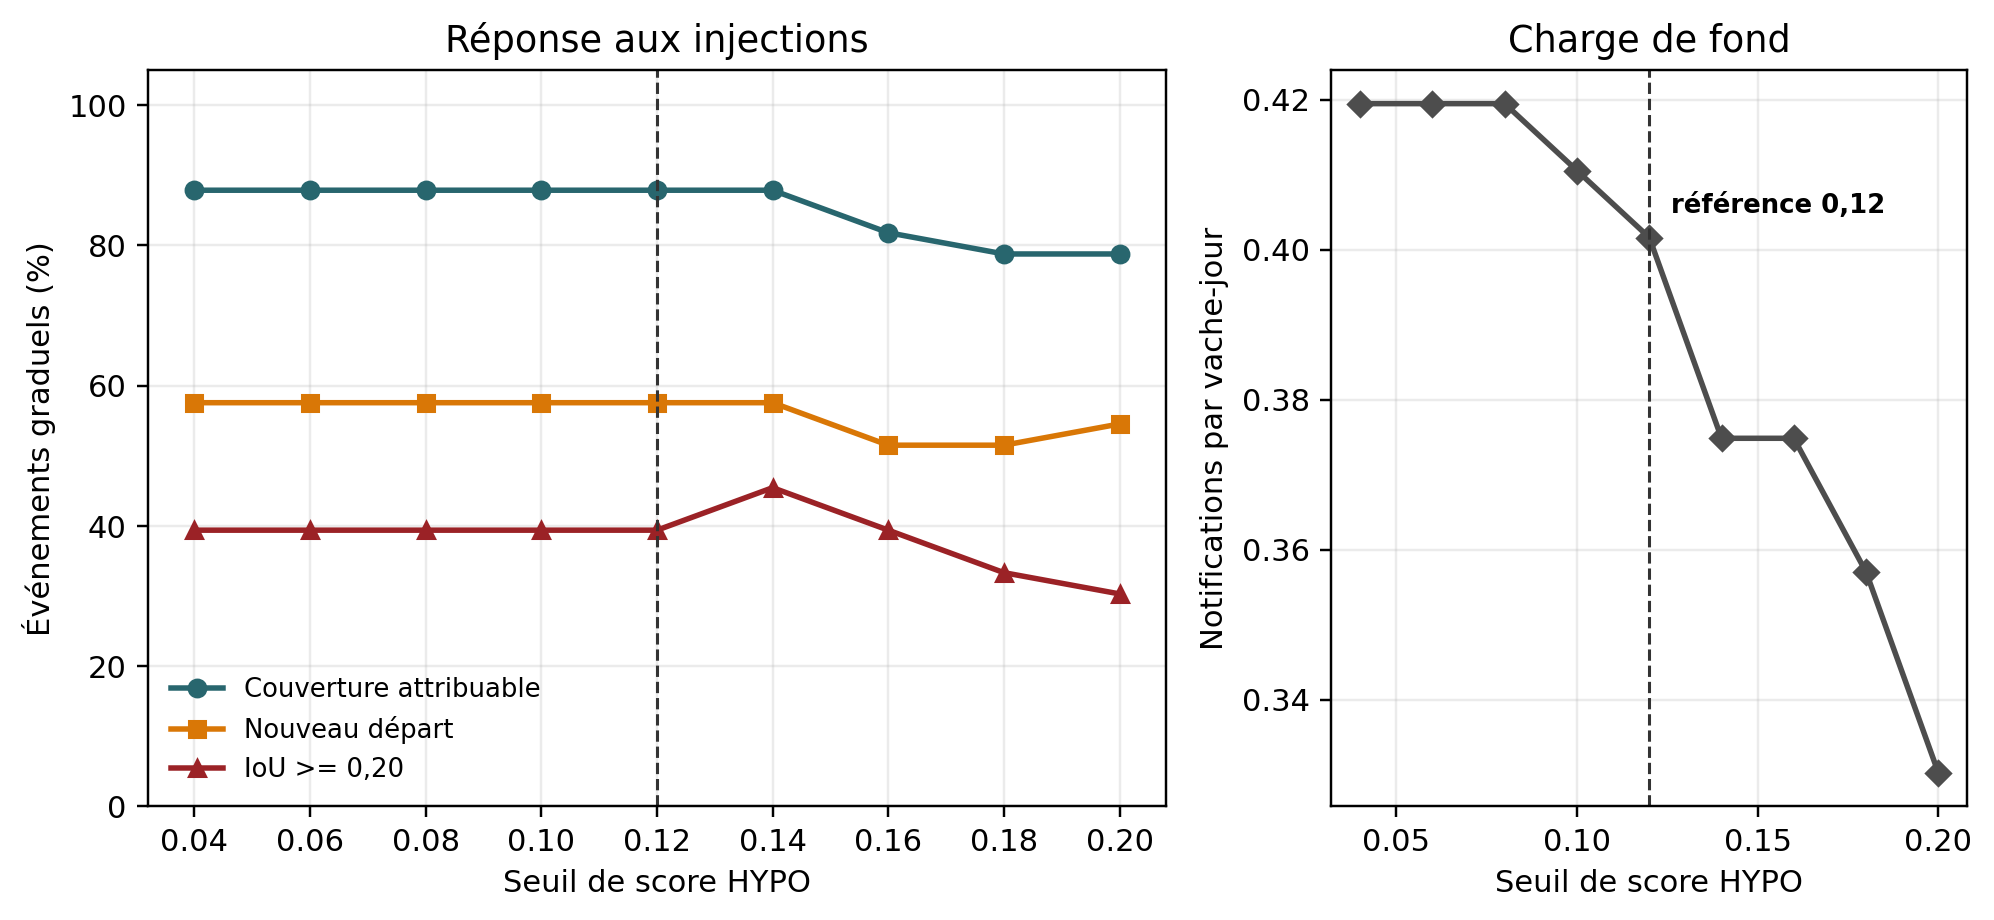
\includegraphics[width=0.98\textwidth]{figures/detection_background_curve.png}
  \caption{Compromis détection-charge de fond.}
  \label{fig:detection_background_curve}
\end{figure}

\subsection{Inspection visuelle ciblée}
La Figure~\ref{fig:manual_review} montre quatre situations de la vache 8081 après le gel
des paramètres. L'hypoactivité modérée produit un épisode de vérification, alors que
l'instabilité modérée reste au niveau de surveillance. Le pic capteur isolé est rejeté et
l'hypoactivité non
locomotrice produit une alerte comparable à celle d'une baisse locomotrice. Dans le premier
panneau, l'épisode est déjà actif à l'ouverture de la fenêtre~: il compte donc comme couverture
attribuable mais non comme nouveau départ, le critère exigeant un début absent de l'exécution
propre. La fenêtre injectée
apparaît en fond gris derrière les courbes, tandis que les sorties du système occupent un
bandeau distinct sous l'axe des signaux~: rouge pour un épisode de vérification, ambre pour une
période de surveillance sans alerte. Le rejet est ainsi la seule issue qui ne reçoit aucune
marque. Séparer la vérité injectée des sorties sur deux canaux distincts évite toute teinte
intermédiaire et rend leur recouvrement directement lisible. Chaque panneau affiche 12
heures de part et d'autre de la fenêtre injectée, et le bandeau rend compte de l'état du
système sur toute la période représentée, marges comprises~; l'issue annoncée dans le titre
porte en revanche sur la seule fenêtre injectée. Une bande de surveillance située hors de
cette fenêtre n'entre pas dans les taux rapportés, qu'elle relève du bruit de fond ou d'une
réaction différée à l'événement injecté comme au panneau du pic capteur, ce qui
explique qu'un panneau puisse en présenter alors que le scénario correspondant affiche un
taux de surveillance nul. Les traits verticaux pointillés
marquent les bornes exactes de la fenêtre injectée, y compris lorsqu'elle ne dure qu'un seul
pas de temps. Dans chaque panneau, les trois
signaux sont tracés bruts en transparence sous une moyenne glissante horaire, et normalisés
séparément par le maximum de cette moyenne : un pic isolé ne comprime donc plus le reste de la
courbe contre l'axe. Cette inspection vérifie la cohérence technique des sorties.

% Page paysage. Le folio normal tomberait sur le bord gauche une fois la page
% pivotee : on le neutralise et on le replace, pivote, au bas de la vue paysage
% pour qu'il se lise comme sur toutes les autres pages. Le flottant est fixe par
% [H] afin que la figure ne se deplace pas d'une compilation a l'autre.
\begin{landscape}
  \thispagestyle{empty}%
  \AddToShipoutPictureFG*{%
    \AtPageLowerLeft{\raisebox{0.5\paperheight}{\makebox[\paperwidth][r]{%
      \rotatebox{90}{\makebox[0pt][c]{\thepage}}\hspace{1.9cm}}}}%
  }%
  \begin{figure}[H]
    \centering
    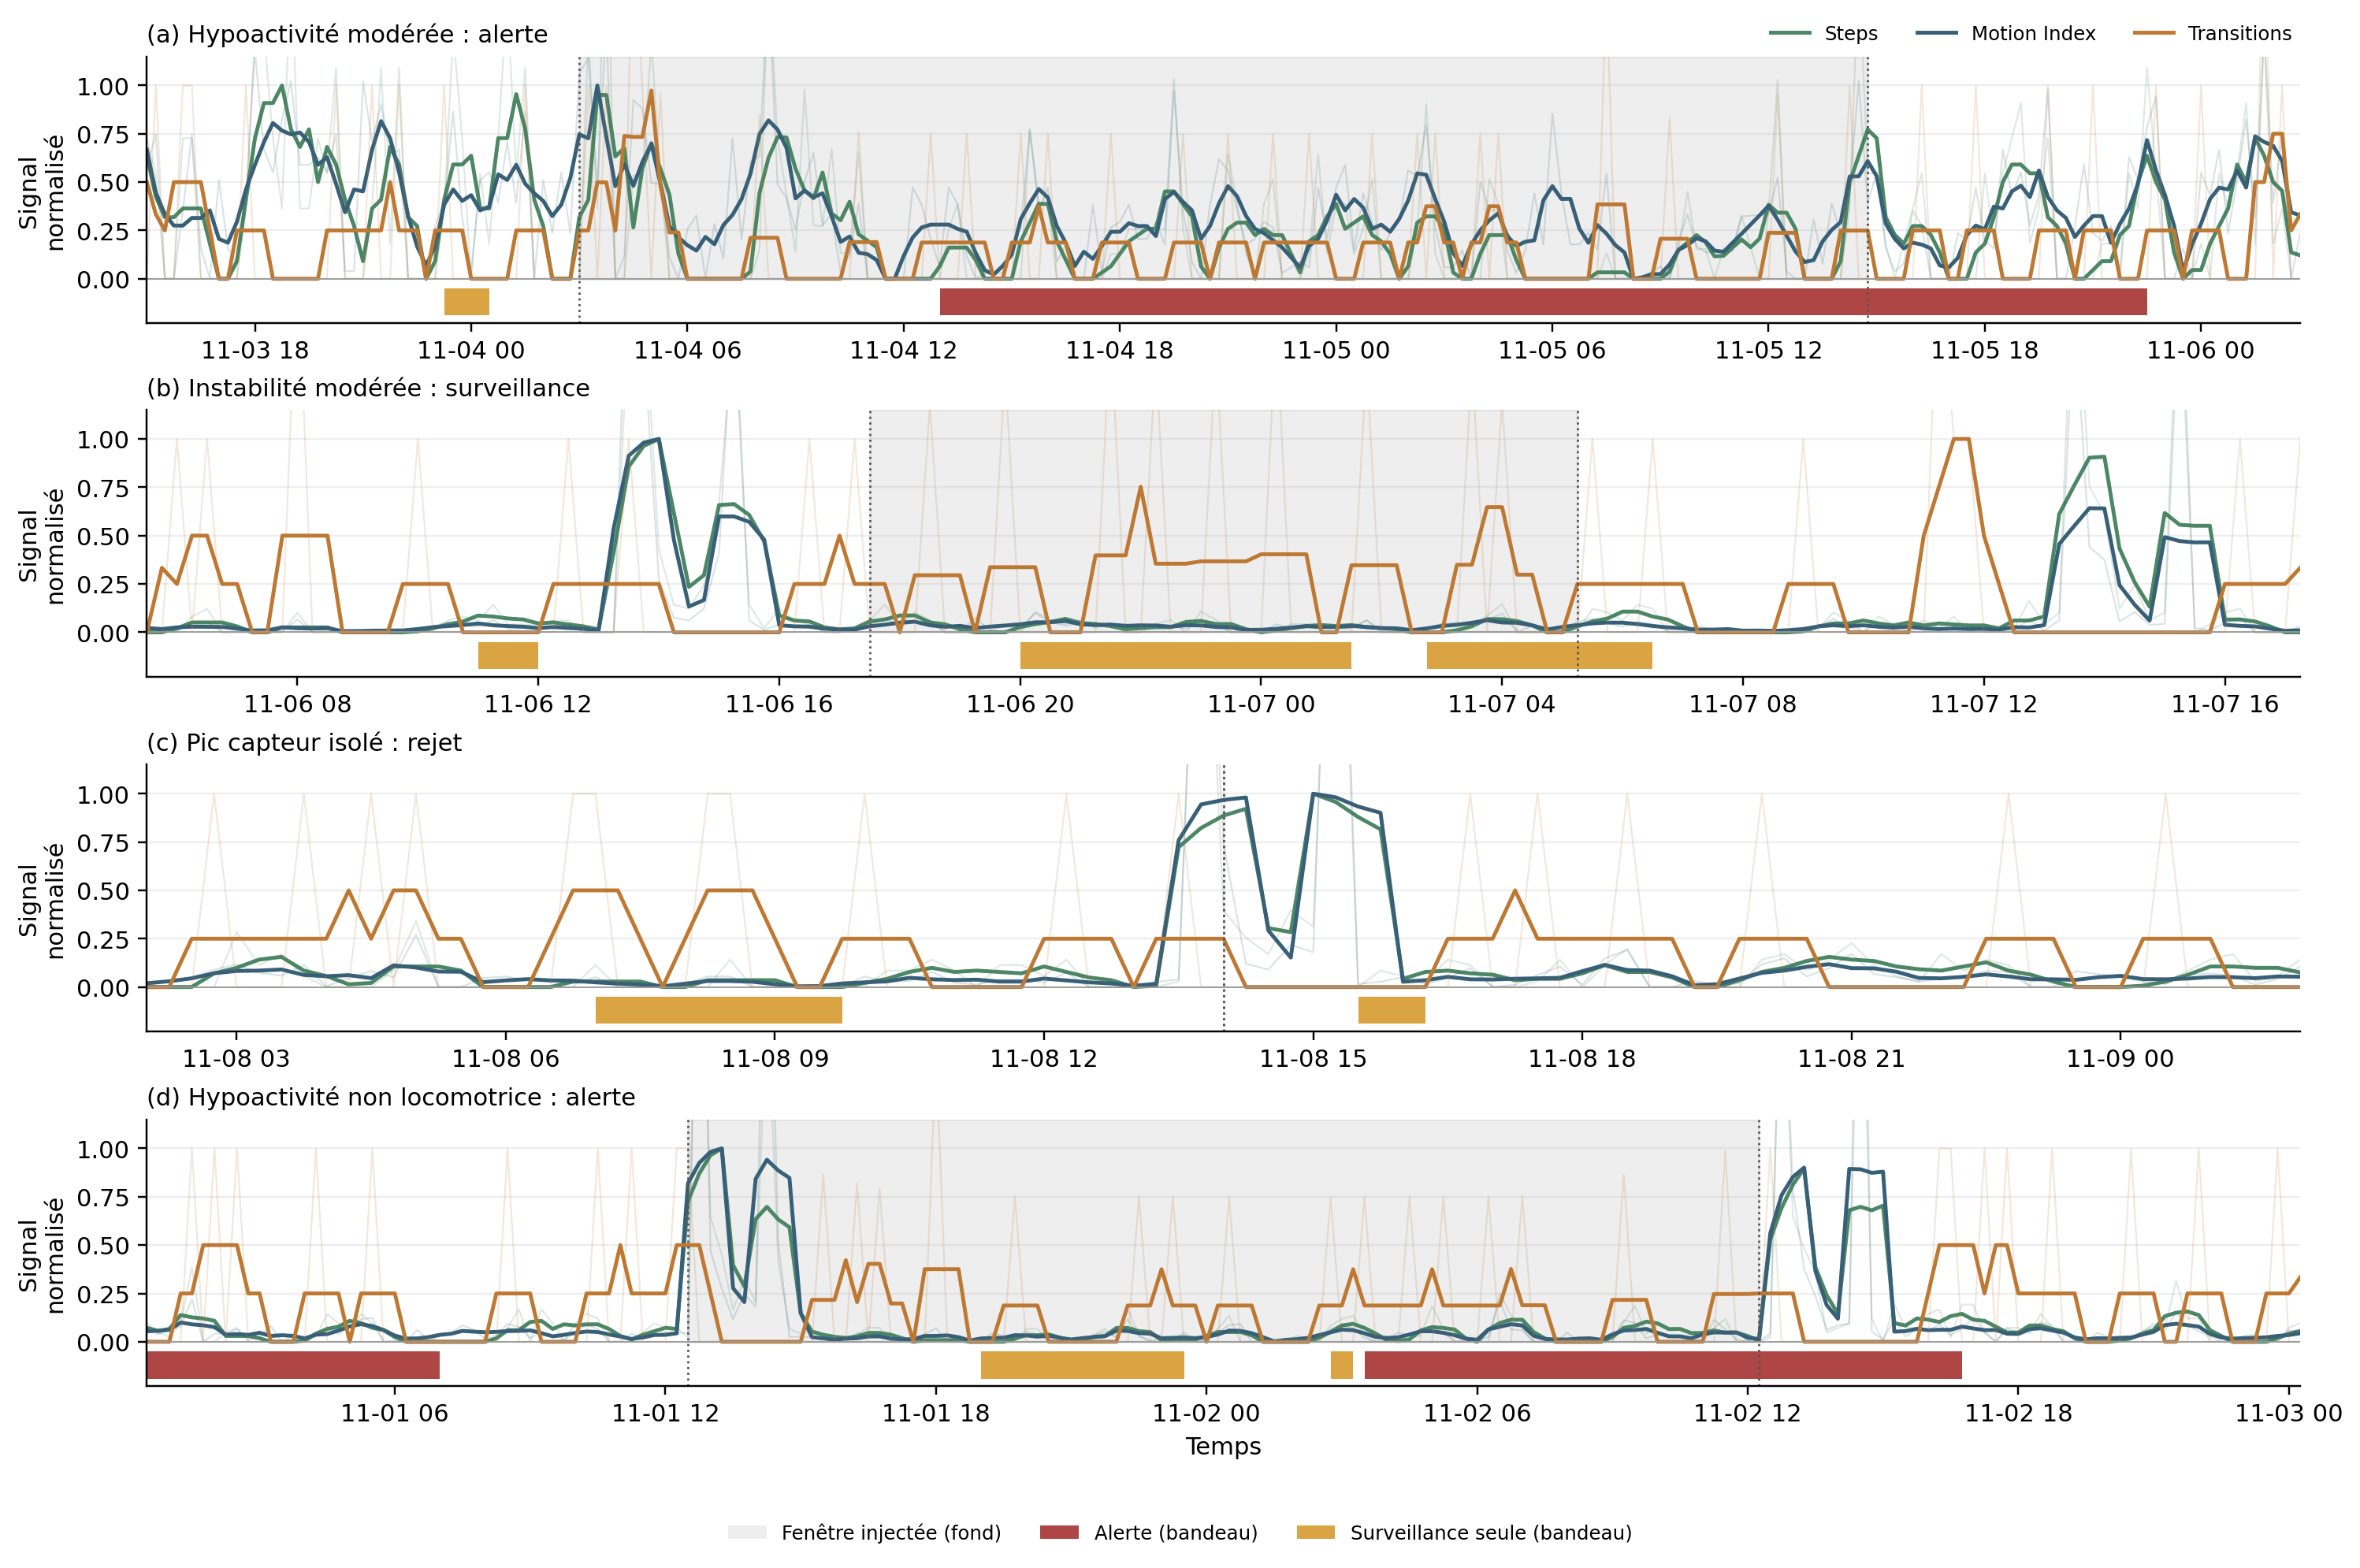
\includegraphics[width=0.95\linewidth]{figures/manual_review.png}
    \caption{Inspection visuelle de scénarios représentatifs.}
    \label{fig:manual_review}
  \end{figure}
\end{landscape}

\subsection{Calibration individuelle exploratoire}
Une calibration simple a été testée pour répondre à la variabilité du fond entre vaches.
Pour chaque vache, le seuil de 0,12 est multiplié par le rapport entre l'écart-type de son
score pendant la période de référence et la médiane de ces écarts-types. Les facteurs, estimés sans utiliser la
période future, restent compris entre 0,98 et 1,03. La procédure laisse inchangés le fond
moyen (0,402 notification par vache-jour), son coefficient de variation inter-vache (0,244)
et la couverture attribuable (87,9\,\%). Le taux de nouveaux départs passe de 57,6 à
60,6\,\%, mais IoU20 diminue de 39,4 à 33,3\,\%. Cette calibration n'apporte donc aucun gain
opérationnel et dégrade la localisation; elle n'est pas retenue. Ce résultat nul ne démontre
pas qu'aucune calibration individualisée soit possible, seulement que la dispersion du
score de référence n'est pas une base utile dans cette campagne.

\subsection{Temps d'exécution}
L'évaluation complète inclut les variables, IF, les règles IF comparatives, HYPO,
INSTABILITÉ, la fusion et la concaténation des sorties. Sur les 28 vaches et 37\,839 lignes,
la médiane de cinq répétitions est de 10,64 secondes, avec une étendue de 10,58 à 10,83
secondes et un débit médian de 3\,557 lignes par seconde. Dans le temps instrumenté, IF
représente 82,8\,\%, les variables 8,2\,\%, HYPO+INSTABILITÉ+fusion 6,4\,\% et les règles IF
comparatives 2,5\,\%. L'extension hybride ajoute donc un coût mesurable mais secondaire par rapport
au comparateur IF. Ces valeurs décrivent la machine de test et ne constituent pas un test de
charge en ferme.

Cette section établit le résultat principal du mémoire~: après soustraction de l'exécution
propre, 29 des 33 dégradations graduelles injectées sont recouvertes, 19 donnent lieu à un
nouvel épisode, et la charge de fond reste sous une notification par vache-jour.

% =====================================================================
\section{Comparaison à IF et LOF, et ablation par le comparateur pédométrique}
% =====================================================================
Les cinq variantes d'ablation sont évaluées sur les mêmes 44 fenêtres. La colonne de détection
attribuable retient le critère de nouveau départ, c'est-à-dire l'apparition d'un épisode
absent de l'exécution propre. La cinquième variante, le comparateur pédométrique, restreint
le détecteur au seul canal des pas, à la manière d'un podomètre. Le
Tableau~\ref{tab:hypo_ablation} rapporte les métriques attribuables des cinq variantes. Le
F1 événementiel y oppose les 33 dégradations graduelles, traitées comme positifs, aux
11 contrôles brefs, traités comme négatifs, sur le critère de nouveau départ attribuable.

\begin{table}[H]
  \centering
  \caption{Ablation attribuable du module HYPO.}
  \label{tab:hypo_ablation}
  \small
  \begin{tabular}{lrrrrr}
    \toprule
    Variante & Nouv. départ & IoU20 & IoU moyen & Fond/vache-jour & F1 \\
    \midrule
    A. HYPO temporel multivarié & 43,2\,\% & 29,5\,\% & 0,137 & 0,402 & 0,73 \\
    B. IF + règles de persistance & 15,9\,\% & 0,0\,\% & 0,004 & 0,152 & 0,35 \\
    C. IF ponctuel & 13,6\,\% & 0,0\,\% & 0,002 & 7,658 & 0,31 \\
    D. LOF + règles & 15,9\,\% & 0,0\,\% & 0,005 & 0,107 & 0,35 \\
    E. Comparateur pédométrique (pas seuls) & 27,3\,\% & 31,8\,\% & 0,141 & 0,518 & 0,53 \\
    \bottomrule
  \end{tabular}
\end{table}

La colonne IoU20 se lit avec le reste du tableau~: le comparateur pédométrique y devance
légèrement le détecteur complet, mais il ouvre moins de nouveaux départs et produit davantage
de fond. Les deux localisent en réalité de
façon équivalente, comme le confirme plus loin l'écart d'IoU attribuable par vache.

La dernière colonne résume la détection et le rejet des contrôles en un F1 événementiel: HYPO atteint
0,73 (IC95 par vache [0,60~; 0,86]), nettement au-dessus d'IF et de LOF (au plus 0,35). Comme
aucun contrôle n'est alerté (précision de 1,0), ce F1 ne fait toutefois que réexprimer le rappel
et n'intègre pas la charge de fond: avec la couverture attribuable, plus permissive que le
nouveau départ, le comparateur pédométrique passerait même devant HYPO sur ce seul résumé, au
prix d'un fond bien plus élevé. Le
F1 reste donc un complément des métriques décomposées et de la charge de fond, qui demeurent
privilégiées.

Après agrégation par vache, HYPO obtient un IoU supérieur aux trois variantes fondées sur IF
et LOF, soit B, C et D
($p=0{,}00098$ pour les trois comparaisons appariées de Wilcoxon~\citep{wilcoxon1945individual}).
Son taux de nouveau départ est également supérieur à B et D ($p=0{,}04297$) et à C
($p=0{,}01562$); ces valeurs sont non corrigées. Après correction de Holm pour les trois
comparaisons, l'avantage d'IoU demeure significatif dans chaque cas ($p_{aj.}=0{,}00294$).
Pour le nouveau départ, seule la comparaison avec C demeure juste sous le seuil
($p_{aj.}=0{,}04686$), tandis que celles avec B et D ne le franchissent plus
($p_{aj.}=0{,}08594$). Ces comparaisons secondaires sont donc interprétées comme
exploratoires. L'avantage est aussi de
\emph{taille}~: l'écart d'IoU attribuable moyen par vache vis-à-vis des comparateurs IF et LOF
est d'environ 0,13 (IC95 [0,106~; 0,161] contre B, [0,107~; 0,163] contre C, [0,103~; 0,161]
contre D, tous excluant zéro), avec une corrélation rang-bisériale appariée
\citep{kerby2014simple} de $+1{,}00$~:
les onze vaches favorisent HYPO. La supériorité ne tient donc pas à quelques vaches.

Cette supériorité appelle une objection, car l'analyse de sensibilité de la
Section~\ref{sec:sensibilite} fait varier 10 paramètres de HYPO et aucun paramètre des
comparateurs. Le paramètre \texttt{contamination} d'Isolation Forest et de LOF, que le
Chapitre~\ref{chapitre:etatart} désigne comme critique pour ces deux méthodes, reste figé à
0,06. L'échec de localisation des comparateurs pourrait donc refléter ce choix plutôt que
leur principe. L'ablation a été rejouée à cinq valeurs de contamination, de 0,02 à 0,15, sur
les mêmes onze vaches et les mêmes quarante-quatre événements. Aucune de ces valeurs ne
permet à B, C ou D d'atteindre le seuil IoU20 sur un seul événement, et leur IoU attribuable
moyen ne dépasse jamais 0,008, contre 0,137 pour HYPO. Ce que la contamination gouverne est
le volume d'alertes et non la localisation~: la charge de fond d'Isolation Forest ponctuel
passe de 2,509 à 14,707 notifications par vache-jour sur cette plage, sans qu'aucun événement
ne soit mieux situé. La valeur retenue ne désavantage donc pas les comparateurs, et l'écart
mesuré tient à la nature de la détection plutôt qu'à un réglage. HYPO et le comparateur
pédométrique, qui n'emploient pas Isolation Forest, restent inchangés sur toute la plage et
servent de témoin à cette vérification.

La cinquième variante isole le rôle de la combinaison de plusieurs signaux. Le comparateur
pédométrique (E) reprend exactement la machinerie temporelle de HYPO (même période de référence
individuelle par créneau horaire, même cumul CUSUM et même persistance), mais restreint la
détection au seul canal des pas, à la manière du comptage d'activité d'un podomètre
\citep{alsaaod2012electronic}; la cohérence entre familles, qu'un canal unique ne peut
satisfaire, y est relâchée pour ne pas le désavantager. Partageant cette machinerie, E
\emph{localise} les épisodes aussi précisément que le détecteur complet~: l'écart d'IoU
attribuable par vache n'est que de $-0{,}004$ (IC95 [$-0{,}032$~; 0,022], $p=0{,}966$, six
vaches sur onze le favorisant légèrement), là où les comparateurs IF et LOF s'effondrent à
un IoU quasi nul. Sa faiblesse est ailleurs~: restreint aux pas, il ouvre moins de nouveaux
    départs attribuables (27,3 contre 43,2~\%) et laisse passer davantage de fond (0,518 contre
    0,402 notification par vache-jour). Le test apparié sur la détection vaut $p=0{,}0625$ et
    n'atteint donc pas le seuil de significativité, mais cette valeur doit se lire avec la
    résolution du test~: chaque vache ne portant que quatre événements, son taux de détection ne
    peut prendre que cinq valeurs, six vaches sur onze sont à égalité exacte et l'effectif
    informatif tombe à cinq paires. Le plancher du test exact bilatéral y vaut précisément
    0,0625, de sorte que cette comparaison ne peut pas être significative à 5~\%, quelle que soit
    l'ampleur de l'écart. Les cinq paires informatives favorisent toutes HYPO. La conclusion
    prudente est donc que la supériorité en détection n'est pas établie faute de résolution, et
    non qu'elle est infirmée. L'écart pédomètre moins HYPO sur le fond atteint 0,116
    notification par vache-jour (IC95 [0,045~; 0,187]); huit vaches sur onze présentent moins de
    fond avec HYPO et le test exact apparié bilatéral vaut $p=0{,}02344$. Cette comparaison de
    fond, ajoutée après examen des autres métriques et non corrigée pour leur multiplicité, reste
    exploratoire. Elle soutient néanmoins une hypothèse utile~: plusieurs signaux pourraient
    réduire la charge de revue sans améliorer la localisation. Elle ne suffit pas à démontrer un
    avantage indépendant de la cohérence multivariée. Ce constat rejoint la limite connue des
approches strictement podométriques, dont la sensibilité dépend du seul comptage de pas
\citep{alsaaod2012electronic,oleary2020accelerometers}.

L'ablation situe donc l'apport du détecteur~: la machinerie temporelle explique l'essentiel de
l'écart avec IF et LOF, tandis que la cohérence multivariée se traduit d'abord par une charge
de vérification plus faible que celle du comparateur pédométrique.

% =====================================================================
\section{Analyses de sensibilité}
% =====================================================================
Les analyses réunies dans cette section examinent la dépendance des conclusions aux familles de signaux
retenues puis aux valeurs de paramètres. Elles évaluent une robustesse locale et ne
sélectionnent aucune nouvelle configuration.

\subsection{Apport de chaque famille de signaux}
Le comparateur pédométrique suggère, pour les pas, que la combinaison de signaux peut réduire la
charge de fond sans changer la localisation. On examine si ce motif descriptif se retrouve
en rejouant la même ablation, mais en restreignant tour à tour le détecteur à chacune
des quatre familles, comme le montre le Tableau~\ref{tab:hypo_channels}. Là où le
Tableau~\ref{tab:hypo_ablation}
situe HYPO face à d'autres familles d'algorithmes (IF, LOF, podomètre), celui-ci décompose ce
qu'il doit à chacune de ses propres familles de signaux; les deux se lisent donc ensemble.
Dans ce test, le détecteur temporel est restreint à un seul canal et la cohérence
multi-familles est relâchée. Le canal des pas correspond au comparateur pédométrique déjà
rapporté comme variante~E du Tableau~\ref{tab:hypo_ablation}.
Chaque canal porte effectivement du signal, et certains,
pris isolément et libérés de la contrainte de cohérence, ouvrent même davantage de nouveaux
départs que le détecteur complet~: les transitions seules atteignent 50,0\,\% (F1 de 0,80) et
le \textit{Motion Index} seul 34,1\,\%. Cette détection brute plus élevée se paie toutefois
exactement où on l'attend, en charge de fond~: les trois canaux d'activité isolés notifient
entre 0,49 et 0,52 fois par vache-jour, contre 0,40 pour HYPO. La posture seule illustre
l'écueil inverse~: son fond est le plus bas (0,384), mais elle ne localise presque rien
(IoU20 de 2,3\,\%). Aucune
famille ne domine donc sur tous les plans. Dans cette campagne, combiner les quatre obtient une
charge de fond basse à localisation comparable et évite de faire dépendre la décision d'un signal
unique susceptible d'être confondu, par exemple les pas gonflés par l'exercice ou l'œstrus. Ce
profil est compatible avec un gain de robustesse par cohérence, mais la résolution insuffisante du
test de détection face au comparateur pédométrique empêche de l'établir comme effet causal
indépendant~: l'écart y va constamment dans le même sens sans pouvoir être certifié.

\begin{table}[H]
  \centering
  \caption{Ablation par famille de signaux.}
  \label{tab:hypo_channels}
  \small
  \begin{tabular}{lrrrrr}
    \toprule
    Canal isolé & Nouv. départ & IoU20 & IoU moyen & Fond/vache-jour & F1 \\
    \midrule
    Pas seuls & 27,3\,\% & 31,8\,\% & 0,141 & 0,518 & 0,53 \\
    Motion Index seul & 34,1\,\% & 25,0\,\% & 0,135 & 0,491 & 0,63 \\
    Transitions seules & 50,0\,\% & 27,3\,\% & 0,128 & 0,518 & 0,80 \\
    Posture seule & 27,3\,\% & 2,3\,\% & 0,042 & 0,384 & 0,53 \\
    HYPO (quatre familles) & 43,2\,\% & 29,5\,\% & 0,137 & 0,402 & 0,73 \\
    \bottomrule
  \end{tabular}
\end{table}

Le calcul de cette ablation par canal est reproductible par
\path{scripts/compute_channel_ablation.py}. Chaque variante retire les autres familles du
score et de l'évidence cumulée par le CUSUM; la ligne « posture seule » ne conserve donc
aucune contribution cachée des pas, du \textit{Motion Index} ou des transitions.

Prises ensemble, les deux ablations (Tableaux~\ref{tab:hypo_ablation} et~\ref{tab:hypo_channels})
soutiennent surtout l'apport de la direction du changement et de la persistance. Elles font de la
cohérence entre signaux une hypothèse crédible de réduction du fond, sans démontrer son apport
indépendant sur la détection ou la localisation. Elles ne résolvent pas la charge opérationnelle,
qui reste supérieure à celle des variantes B et D.

\subsection{Robustesse locale des paramètres HYPO}
\label{sec:sensibilite}
L'analyse OFAT comprend la référence et 20 variantes de paramétrage dans lesquelles un
seul des dix
paramètres est modifié. Les 924 évaluations événement-configuration rejettent toutes le
contrôle bref. Sur les profils progressifs, 12 variantes sur 20 reproduisent exactement le
taux de nouveaux départs de la référence et 15 restent dans un écart maximal de 6,1 points.
Pour IoU20, 15 variantes restent dans un écart maximal de 3,0 points. Sur l'ensemble des
valeurs testées, le taux de nouveaux départs varie de 45,5 à 66,7\,\%, la couverture de
63,6 à 90,9\,\%, IoU20 de 27,3 à 45,5\,\%, le délai médian de 15,5 à 24,5 heures et le fond
de 0,187 à 0,553 notification par vache-jour.

La Figure~\ref{fig:hypo_sensitivity} représente l'amplitude maximale de ces écarts. Elle
mesure une influence locale des paramètres, et non une amélioration ou une optimisation de
la configuration de référence. Le panneau~(a) rapporte l'amplitude des écarts sur les
événements progressifs, le panneau~(b) celle observée sur la charge de fond. Le
Tableau~\ref{tab:hypo_sensitivity} en détaille les plages
signées pour les paramètres les plus structurants.

\begin{figure}[H]
  \centering
  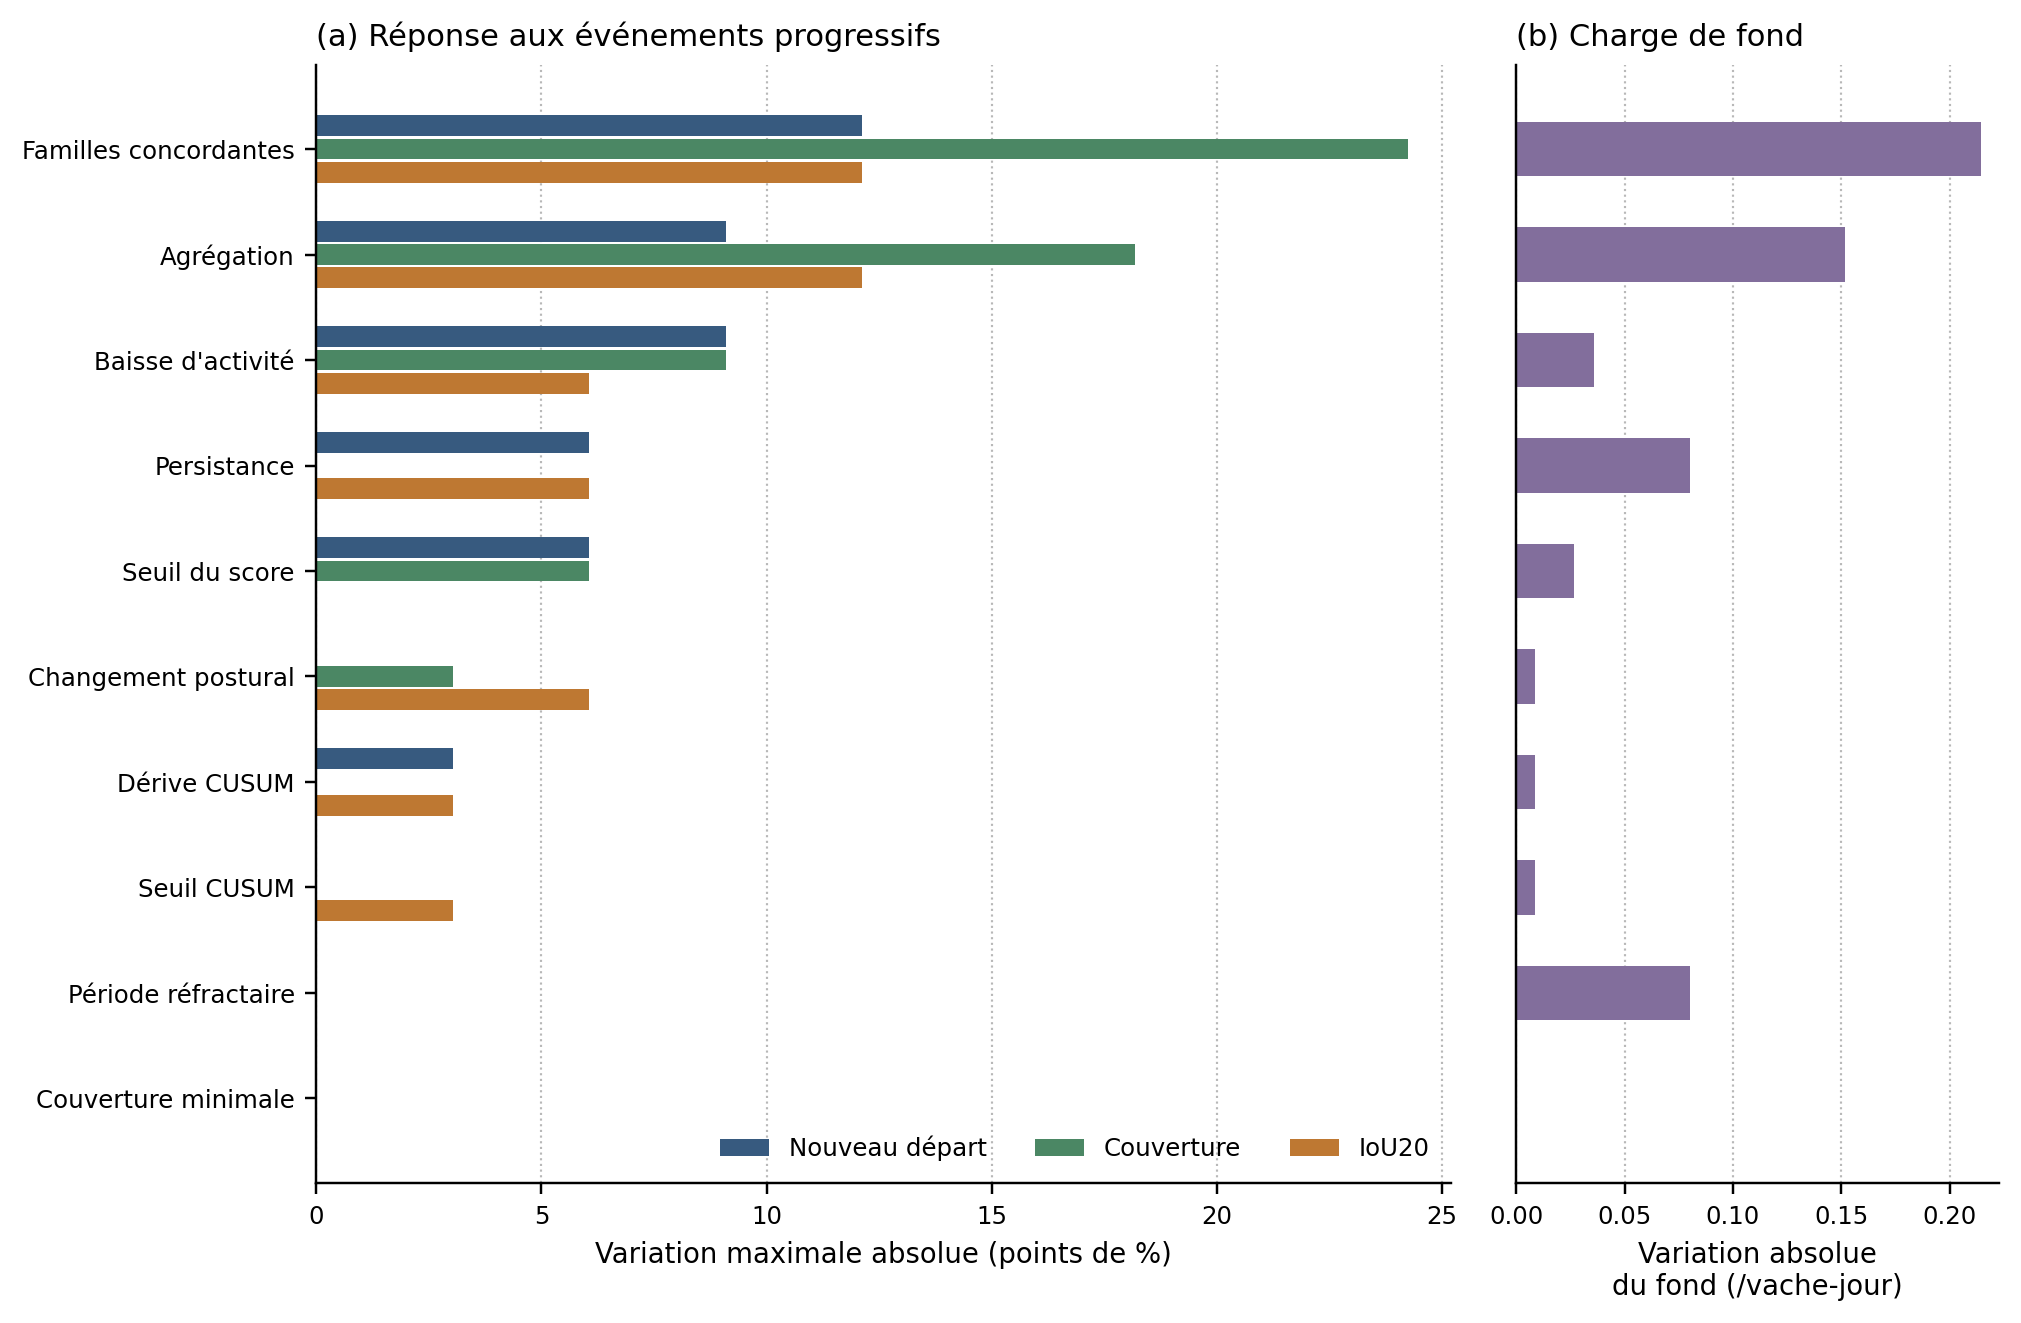
\includegraphics[width=0.98\textwidth]{figures/hypo_parameter_sensitivity_effects.png}
  \caption{Sensibilité locale des paramètres HYPO.}
  \label{fig:hypo_sensitivity}
\end{figure}

\begin{table}[H]
  \centering
  \caption{Plages d'écarts signés pour les paramètres HYPO les plus structurants.}
  \label{tab:hypo_sensitivity}
  \small
  \setlength{\tabcolsep}{3pt}
  \begin{tabular}{p{0.20\textwidth}p{0.10\textwidth}
    >{\centering\arraybackslash}p{0.13\textwidth}
    >{\centering\arraybackslash}p{0.15\textwidth}
    >{\centering\arraybackslash}p{0.12\textwidth}
    >{\centering\arraybackslash}p{0.15\textwidth}}
    \toprule
    Paramètre & Valeurs & $\Delta$ départ & $\Delta$ couverture & $\Delta$ IoU20 & $\Delta$ fond \\
      & testées & (pp) & (pp) & (pp) & (/vache-jour) \\
    \midrule
    Familles concordantes & 2; 4 & $-12{,}1$ à $0{,}0$ & $-24{,}2$ à $+3{,}0$ & $-12{,}1$ à $+3{,}0$ & $-0{,}214$ à $+0{,}107$ \\
    Agrégation & 6; 24 h & $-9{,}1$ à $+9{,}1$ & $-18{,}2$ à $0{,}0$ & $-12{,}1$ à $-3{,}0$ & $-0{,}098$ à $+0{,}152$ \\
    Baisse d'activité & 5; 15\,\% & $-9{,}1$ à $-9{,}1$ & $-9{,}1$ à $+3{,}0$ & $-6{,}1$ à $-3{,}0$ & $-0{,}036$ à $+0{,}027$ \\
    Persistance & 3; 12 h & $-6{,}1$ à $0{,}0$ & $0{,}0$ à $0{,}0$ & $-3{,}0$ à $+6{,}1$ & $-0{,}054$ à $+0{,}080$ \\
    \bottomrule
  \end{tabular}
\end{table}

Le nombre de familles et la fenêtre d'agrégation sont les choix les plus influents. Les
paramètres CUSUM et de couverture ont peu d'effet dans les plages testées. Cette stabilité
locale rend la configuration reproductible et techniquement défendable, mais ne démontre
ni son optimalité ni sa validité physiologique.

\subsection{Sensibilité des paramètres INSTABILITÉ}
Trois variantes proches sont comparées à la référence. La détection des scénarios de vérification reste entre
72,7 et 75,0\,\%, tandis que la surveillance varie de 54,5 à 66,7\,\% et le fond de 0,518 à
0,571 notification par vache-jour. Une persistance de trois heures réduit la surveillance
et augmente les confusions; une agrégation de quatre heures réduit également la surveillance.
Cette analyse soutient la stabilité locale de l'extension, mais elle est beaucoup moins
complète que l'OFAT de HYPO et ne valide pas les seuils physiologiquement.

Sur l'ensemble des 20 variantes, le contrôle bref reste rejeté sans exception~: la conclusion
de la campagne principale ne dépend donc pas d'un seuil isolé.

% =====================================================================
\section{Stress test HYPO à aire d'enveloppe appariée}
% =====================================================================
La campagne gelée applique six formes à trois positions chez chacune des onze vaches, soit
198 événements physiques et 990 évaluations pour les cinq variantes. Les cinq formes
positives modifient plusieurs familles; le contrôle négatif modifie uniquement les pas.
Chaque famille perturbée reçoit une aire numérique d'enveloppe de 36 heures, identique à celle du
profil graduel modéré de référence. Ce contrôle est satisfait pour tous les événements, avec
une erreur relative maximale inférieure à $4\times10^{-16}$. Aucun paramètre du détecteur
n'est modifié après le gel du protocole. L'appariement porte sur l'enveloppe numérique; il ne
garantit pas une variation comportementale physique identique entre vaches ou entre familles.

\begin{table}[H]
  \centering
  \caption{Réponse de HYPO aux formes moins favorables à aire d'enveloppe appariée.}
  \label{tab:hypo_stress}
  \small
  \begin{tabular}{lrrrr}
    \toprule
    Forme & $n$ & Couverture (\%) & Nouveau départ (\%) & IoU20 (\%) \\
    \midrule
    Départ abrupt & 33 & 93,9 & 54,5 & 27,3 \\
    Familles désynchronisées & 33 & 100,0 & 72,7 & 30,3 \\
    Récupération asymétrique & 33 & 93,9 & 63,6 & 21,2 \\
    Graduel bruité & 33 & 97,0 & 66,7 & 51,5 \\
    Bloc manquant de 12 h & 33 & 100,0 & 100,0 & 24,2 \\
    Pas seuls (contrôle) & 33 & 78,8 & 30,3 & 0,0 \\
    \bottomrule
  \end{tabular}
\end{table}

Le Tableau~\ref{tab:hypo_stress} détaille la réponse forme par forme.
Sur les 165 événements positifs, la moyenne des cinq taux par forme atteint 97,0\,\% de
couverture attribuable, 71,5\,\% de nouveaux départs et 30,9\,\% à IoU20. HYPO conserve
donc une forte couverture lorsque la forme s'écarte du profil graduel concordant, mais sa
localisation demeure modeste et varie selon la forme. Le bloc de données manquantes ne doit
pas être interprété comme favorable en soi: la métrique de couverture crédite tout
recouvrement attribuable, alors qu'IoU20 reste à 24,2\,\%.

\begin{table}[H]
  \centering
  \caption{Comparaisons appariées sur les cinq formes positives du stress test.}
  \label{tab:hypo_stress_comparisons}
  \small
  \begin{tabular}{lrr}
    \toprule
    Comparateur & Différence de couverture & $p$ exact unilatéral \\
    \midrule
    IF + persistance & +0,842 & 0,000488 \\
    IF ponctuel & +0,527 & 0,000488 \\
    LOF + persistance & +0,703 & 0,000488 \\
    Pédométrique, pas seuls & $-0,012$ & 0,843750 \\
    \bottomrule
  \end{tabular}
\end{table}

Les tests exacts du Tableau~\ref{tab:hypo_stress_comparisons} utilisent la moyenne de chaque
vache, et non les 165 lignes comme
observations indépendantes. Portant sur onze vaches, ils disposent de $2^{11}=2048$
permutations et d'un plancher unilatéral de 0,000488~: contrairement à la comparaison de détection de la
section précédente, leur absence de conclusion face au comparateur pédométrique n'est pas un
manque de résolution. HYPO conserve un avantage net sur IF et LOF, mais aucun avantage
n'est démontré face au comparateur pédométrique doté de la même machinerie temporelle. De
plus, le contrôle pas-seuls échoue au critère principal de spécificité~: il présente un
recouvrement attribuable dans 78,8\,\% des cas et produit un nouveau départ dans 30,3\,\%.
Le côté favorable est que ces épisodes localisent mal la fenêtre~: aucun n'atteint IoU20 et
l'IoU moyen n'est que de 0,038.

La comparaison des variantes sur ce même contrôle précise toutefois la portée de cet échec.
Le comparateur pédométrique, restreint au canal perturbé, recouvre la fenêtre dans 100,0\,\%
des cas, ouvre un nouveau départ dans 57,6\,\% et atteint IoU20 dans 54,5\,\%~: il localise
donc correctement une perturbation mono-famille. Le détecteur multivarié, lui, n'y parvient
jamais. Sur les 165 événements positifs, les deux restent proches, à 97,0 contre 98,2\,\% de
recouvrement et 30,9 contre 33,9\,\% à IoU20. L'exigence de concordance entre familles ne
supprime donc pas le déclenchement sur un canal isolé, mais elle empêche de le localiser~;
c'est la seule dimension où sa contribution propre se manifeste dans ce stress test. IF et LOF
rejettent ce contrôle plus franchement, à 0,0\,\% de recouvrement pour les variantes dotées de
règles de persistance et 12,1\,\% pour IF ponctuel, mais au prix d'un recouvrement de 12,7 à
44,2\,\% seulement sur les événements positifs.

Le stress test établit ainsi une robustesse temporelle positive face aux cinq formes moins
favorables et un avantage net sur IF et LOF, tout en délimitant précisément l'apport de la
cohérence multivariée~: démontré sur la localisation d'un stimulus mono-famille, non démontré
sur le déclenchement. Avec les signaux disponibles, une vérification contextuelle reste
nécessaire.

% =====================================================================
\section{Extension bidirectionnelle exploratoire}
% =====================================================================
\subsection{Comparaison des règles de fusion}
Le Tableau~\ref{tab:fusions} compare les cinq stratégies sur 132 scénarios. La colonne
« vérification » regroupe les trois scénarios HYPO et la séquence. La surveillance mesure le
recouvrement des trois instabilités. Les facteurs confondants regroupent l'activité de type
œstrus et l'hypoactivité non locomotrice.

\begin{table}[H]
  \centering
  \caption{Comparaison exploratoire des règles de fusion sur 132 événements.}
  \label{tab:fusions}
  \small
  \begin{tabular}{lrrrrr}
    \toprule
    Configuration & Vérification & Surveillance & Confondants & IoU20 & Fond \\
     & (\%) & instabilité (\%) & alertés (\%) & (\%) & /vache-jour \\
    \midrule
    HYPO & 61,4 & 66,7 & 40,9 & 29,5 & 0,446 \\
    INSTABILITÉ & 38,6 & 66,7 & 0,0 & 0,0 & 0,875 \\
    OU & 65,9 & 66,7 & 31,8 & 11,4 & 0,982 \\
    \textbf{HIÉRARCHIQUE} & \textbf{72,7} & \textbf{66,7} & 40,9 & \textbf{29,5} & 0,571 \\
    SÉQUENTIELLE & 56,8 & 66,7 & 36,4 & 0,0 & \textbf{0,366} \\
    \bottomrule
  \end{tabular}
\end{table}

Dans cette comparaison, toutes les sorties fusionnées utilisent un délai réfractaire commun
de 12 heures. Le fond HYPO de 0,446 diffère donc du 0,402 de la campagne principale,
où la notification propre à HYPO est espacée de 24 heures. Les valeurs ne doivent pas être
comparées comme si seul l'algorithme avait changé.

La fusion hiérarchique augmente la couverture des scénarios de vérification par rapport à HYPO seul, conserve
IoU20 à 29,5\,\%, mais élève le fond de 0,446 à 0,571. Sa fonction d'utilité technique reste
négative ($-0{,}088$), car les pénalités de confusion et de charge sont importantes. Elle est
retenue comme configuration représentative de l'extension, non comme remplacement démontré
de HYPO. La Figure~\ref{fig:fusions} compare les cinq règles de fusion.

\begin{figure}[H]
  \centering
  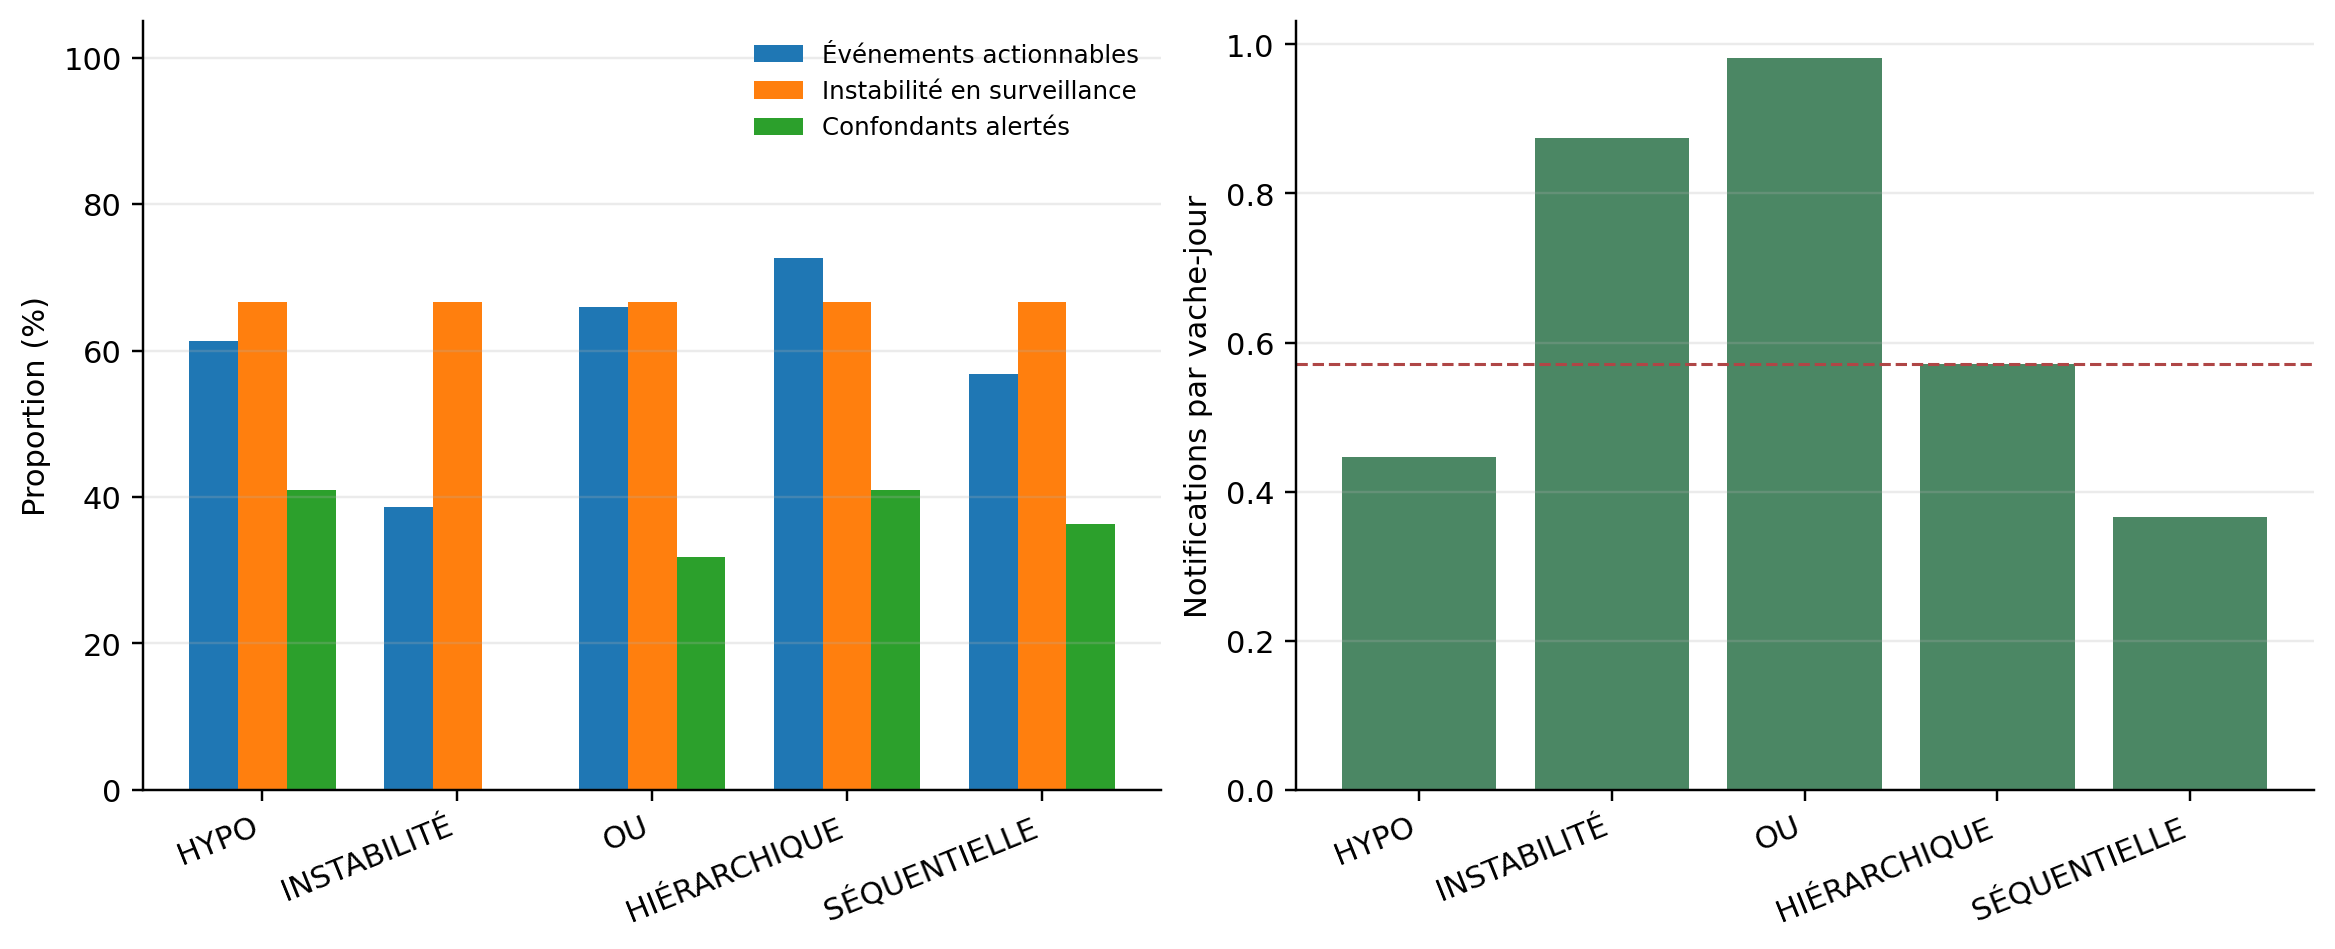
\includegraphics[width=0.92\textwidth]{figures/fusion_comparison.png}
  \caption{Comparaison des règles de fusion.}
  \label{fig:fusions}
\end{figure}

\subsection{Réponse par scénario}
La fusion hiérarchique couvre 45,5\,\% des hypoactivités légères, 72,7\,\% des modérées et
81,8\,\% des marquées. L'instabilité légère, modérée et marquée est observée en surveillance
dans respectivement 45,5\,\%, 54,5\,\% et 100,0\,\% des cas. La séquence synthétique
instabilité-hypoactivité est alertée dans 90,9\,\% des cas. Le Tableau~\ref{tab:scenarios}
détaille ces réponses par scénario, que la Figure~\ref{fig:scenarios} représente
visuellement.

\begin{table}[H]
  \centering
  \caption{Réponse de la fusion hiérarchique par scénario.}
  \label{tab:scenarios}
  \small
  \begin{tabular}{lrrr}
    \toprule
    Scénario & $n$ & Alerte de vérification (\%) & Surveillance (\%) \\
    \midrule
    Hypoactivité légère & 11 & 45,5 & 0,0 \\
    Hypoactivité modérée & 11 & 72,7 & 18,2 \\
    Hypoactivité marquée & 11 & 81,8 & 54,5 \\
    Instabilité légère & 11 & 9,1 & 45,5 \\
    Instabilité modérée & 11 & 9,1 & 54,5 \\
    Instabilité marquée & 11 & 18,2 & 100,0 \\
    Instabilité puis hypoactivité & 11 & 90,9 & 81,8 \\
    Contrôles brefs regroupés & 33 & 0,0 & 0,0 \\
    Activité de type œstrus & 11 & 0,0 & 0,0 \\
    Hypoactivité non locomotrice & 11 & 81,8 & 0,0 \\
    \bottomrule
  \end{tabular}
\end{table}

\begin{figure}[H]
  \centering
  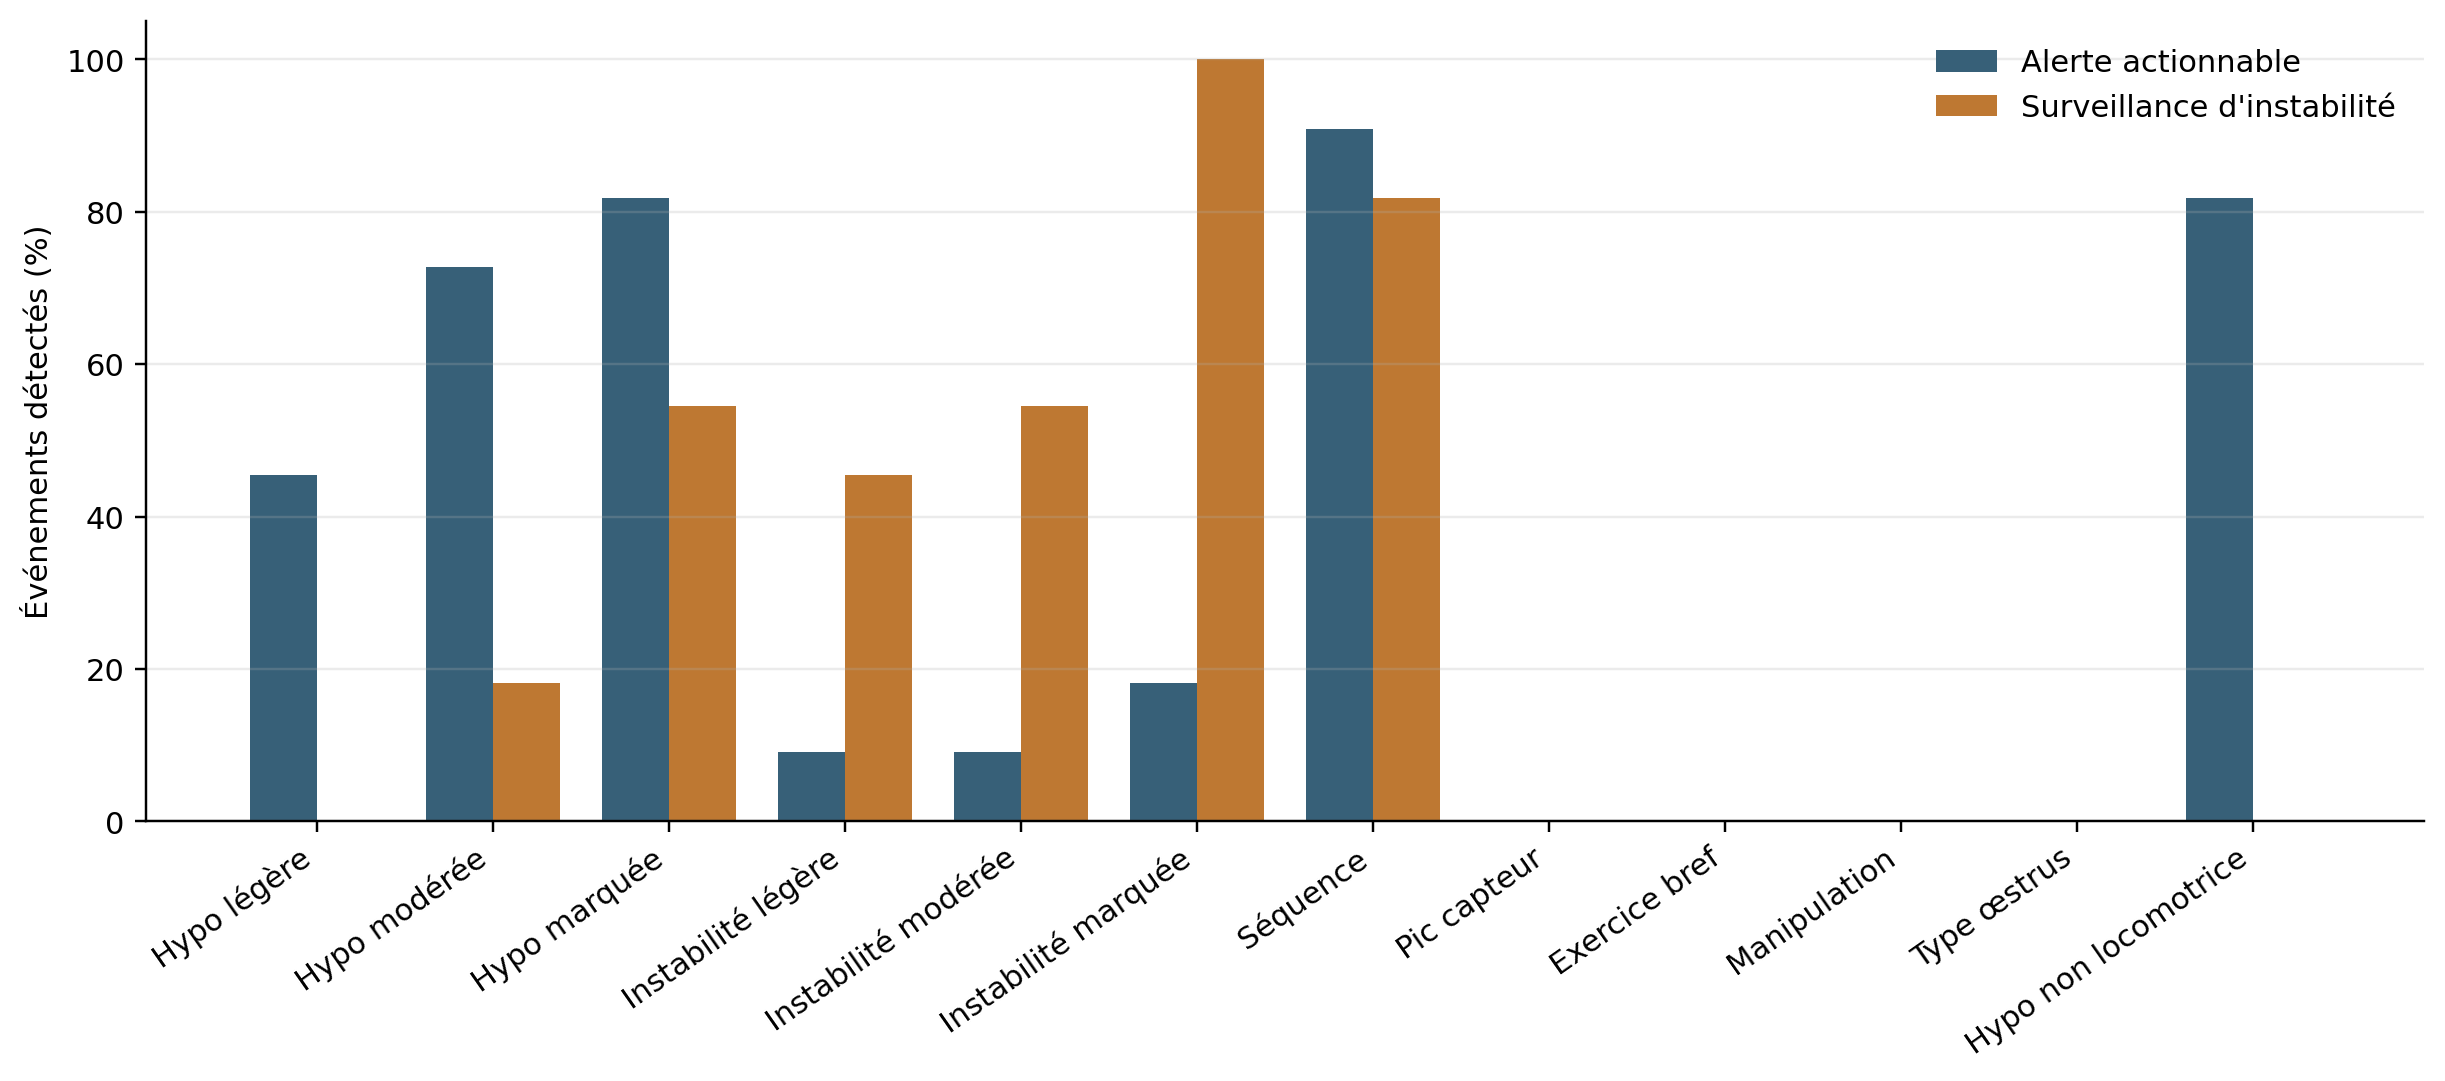
\includegraphics[width=0.94\textwidth]{figures/scenario_results.png}
  \caption{Réponse par scénario contrôlé.}
  \label{fig:scenarios}
\end{figure}

Parmi les scénarios de vérification, 29,5\,\% atteignent IoU20. Le délai médian est de
19,875 heures. Le fond hiérarchique est de 0,571 notification par vache-jour, avec une
étendue de 0,295 à 0,884 entre vaches. Aucun des 33 contrôles brefs ne produit de nouveau
départ de vérification ou de surveillance. Par ailleurs, l'alerte de neuf hypoactivités non
locomotrices sur onze démontre une limite d'identifiabilité:
des causes différentes peuvent produire la même forme sur les capteurs disponibles.

L'extension apporte ainsi une surveillance des instabilités que HYPO seul ne produit pas, sans
améliorer la localisation ni réduire la charge~: elle complète le détecteur principal plutôt
qu'elle ne le remplace.

% =====================================================================
\section{Évaluation observationnelle IceTag-SLS}
% =====================================================================
\label{sec:validation_mcgill}

Quatorze vaches sont évaluables. Les trois vaches SLS~$\geq2$ appartiennent toutes au groupe
\textit{Exercise}; aucune vache du groupe sans exercice n'atteint ce seuil. Dans les sept
jours précédant le score, la fusion hiérarchique produit en moyenne 6,67 notifications chez
les trois vaches SLS~$\geq2$, contre 4,45 chez les onze autres. L'AUC exploratoire est
0,924. L'énumération exhaustive des 364 répartitions possibles des trois étiquettes positives
donne $p=0{,}019$ en unilatéral et $p=0{,}030$ en bilatéral, en accord avec le test de
Mann-Whitney ($p=0{,}031$). La corrélation de Spearman vaut $\rho=0{,}504$ avec
$p=0{,}066$. Chaque point de la Figure~\ref{fig:sls} représente une vache; l'effectif de
trois vaches dans le groupe SLS~$\geq2$ impose une interprétation prudente.

Deux contrôles précisent ce résultat positif. D'abord, retirer successivement chacune des trois
vaches SLS~$\geq2$ maintient l'AUC globale entre 0,909 et 0,955~: le classement n'est donc pas
porté par une seule vache. Ensuite, le test max-stat exact reste favorable lorsqu'il contrôle
les cinq variantes de fusion pour la mesure de notifications ($p=0{,}0467$ en unilatéral).
Lorsqu'il englobe les vingt combinaisons variante-métrique examinées, il devient non concluant
($p=0{,}0742$ en unilatéral et $p=0{,}1236$ en bilatéral). Le signal favorable est donc
spécifique au nombre de notifications et suffisamment stable pour justifier une étude plus
grande, mais il ne constitue pas une confirmation familiale sur toutes les analyses explorées.
Ce contrôle de multiplicité ayant été ajouté après l'analyse principale, il demeure lui-même
exploratoire.

\begin{figure}[H]
  \centering
  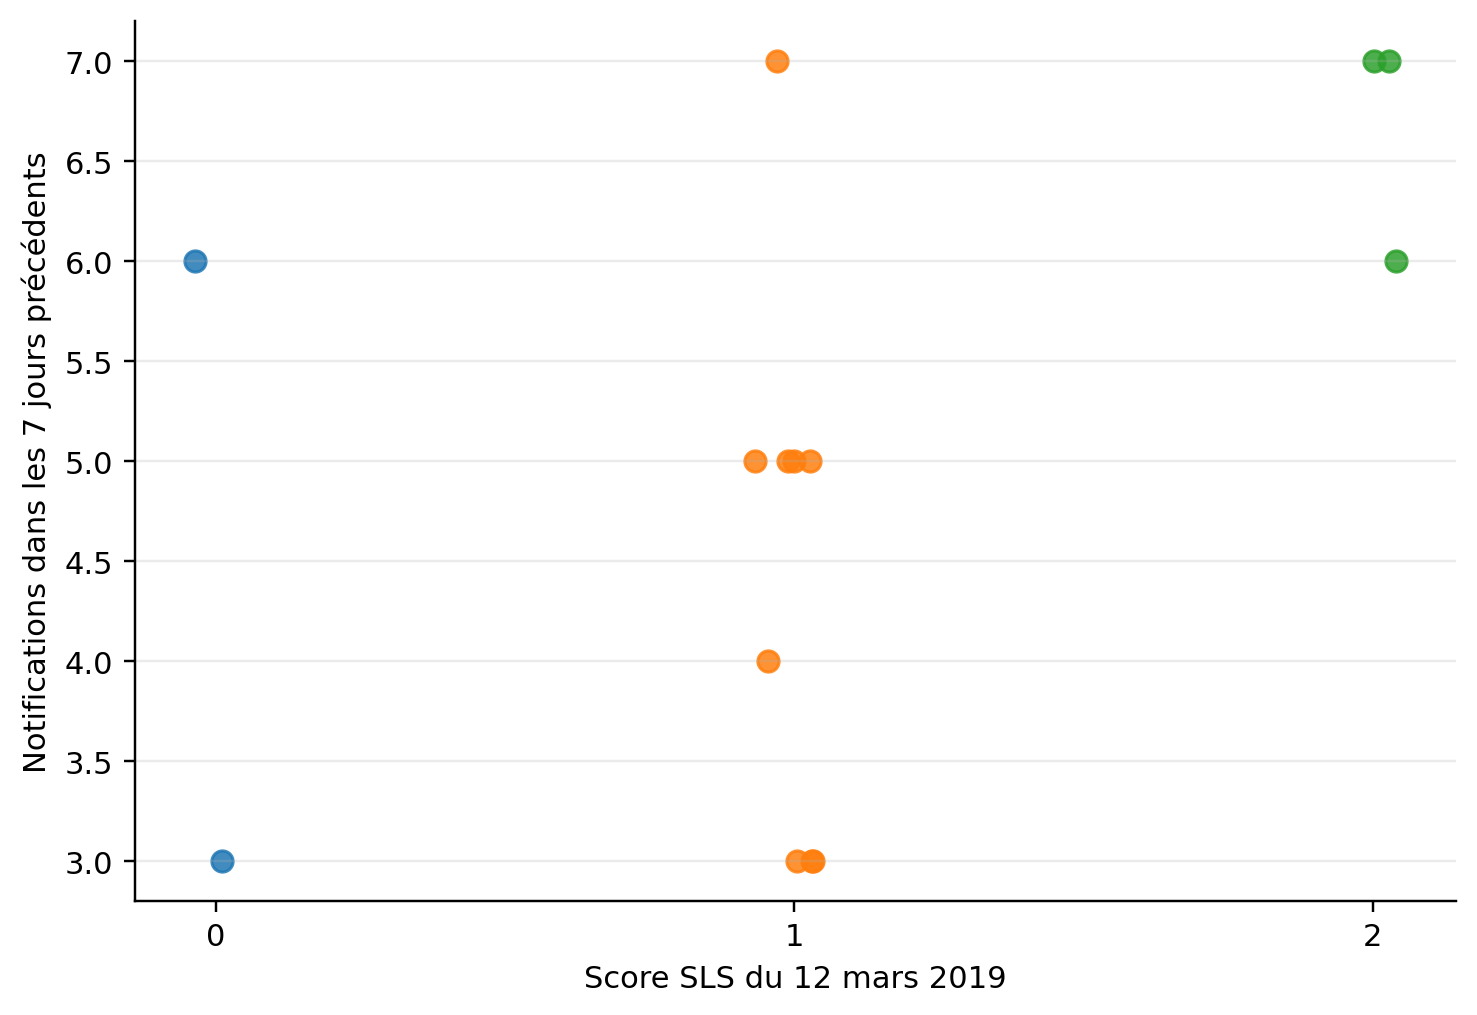
\includegraphics[width=0.72\textwidth]{figures/sls_notifications.png}
  \caption{Notifications précédant le score SLS.}
  \label{fig:sls}
\end{figure}

Les mesures secondaires sont moins séparatrices: l'AUC de la fraction du temps en épisode
est 0,712, celle du score maximum 0,606 et celle de la surveillance d'instabilité 0,348. La
charge future atteint environ 0,755 notification par vache-jour. L'ensemble forme un signal
de concordance intéressant. Cependant, les trois vaches SLS~$\geq2$ se trouvent dans le
groupe \textit{Exercise}, contre trois des dix vaches sous le seuil dont le traitement est
connu; le test exact de Fisher donne $p=0{,}070$. Dans le seul groupe
\textit{Exercise}, l'AUC reste orientée dans le même sens (0,778), mais le test exact
bilatéral est non concluant ($p=0{,}40$). Comme pour la détection face au comparateur
pédométrique, cette absence de conclusion tient d'abord à la résolution~: six vaches réparties
en trois positives et trois négatives n'autorisent que vingt permutations, et le plancher du
test exact bilatéral y vaut 0,10. Ce test ne pouvait donc pas être significatif à 5~\%. Le
groupe sans exercice ne contient aucun cas
SLS~$\geq2$, donc aucune AUC interne n'y est estimable. Malgré la stabilité du classement
global au retrait d'une vache positive, sa portée clinique demeure limitée par le petit
effectif, la multiplicité et la confusion avec le traitement.

Le classement global reste néanmoins net, avec une AUC de 0,924~: c'est la seule confrontation
à des scores locomoteurs réels dont dispose ce travail, et elle va dans le sens attendu.

% =====================================================================
\section{Correspondance entre objectifs et résultats}
% =====================================================================
Le Tableau~\ref{tab:objectifs_resultats} vérifie qu'aucun objectif annoncé dans
l'introduction ne reste sans résultat et qu'aucun résultat principal n'est introduit sans
objectif préalable.

\begin{table}[H]
  \centering
  \caption{Correspondance entre objectifs et résultats.}
  \label{tab:objectifs_resultats}
  \small
  \begin{tabular}{p{0.05\textwidth}p{0.25\textwidth}p{0.42\textwidth}p{0.13\textwidth}}
    \toprule
    Obj. & Attente & Résultat principal & Statut \\
    \midrule
    1 & Référence individuelle et chronologique
      & Séparation 60/40, référence par vache et créneau, contrôles d'intégrité conformes.
      & Réalisé \\
    2 & Détection HYPO persistante
      & 87,9\,\% de couverture attribuable et 39,4\,\% à IoU20 sur 33 profils graduels.
      & Réalisé \\
    3 & Ablation et sensibilité HYPO
      & Supériorité sur IF/LOF; OFAT de 20 variantes; forte couverture des formes de stress
        à aire d'enveloppe appariée, mais contrôle pas-seuls non rejeté sur le recouvrement.
      & Réalisé \\
    4 & Explorer INSTABILITÉ et les fusions
      & Surveillance de 22/33 instabilités; aucune supériorité de la fusion sur HYPO.
      & Exploratoire \\
    5 & Contrôles, confondants, fond et coût
      & Contrôles brefs rejetés, 9/11 hypoactivités non locomotrices alertées,
        fond HYPO de 0,402 et temps médian de 10,64~s.
      & Réalisé \\
    6 & Confrontation IceTag-SLS
      & AUC globale de 0,924; analyse interne au groupe \textit{Exercise} non concluante
        (AUC 0,778; test exact bilatéral $p=0{,}40$).
      & Exploratoire \\
    \bottomrule
  \end{tabular}
\end{table}

La campagne principale établit que HYPO transforme des baisses graduelles injectées après
la période de référence en épisodes attribuables, mieux localisés que ceux des comparateurs IF
et LOF. Le contrôle bref est rejeté, l'ablation favorise HYPO chez les onze vaches, et l'OFAT
montre que la conclusion ne dépend pas d'un seul seuil isolé. Le comparateur pédométrique
localise de façon proche, mais recouvre moins d'événements et produit plus de fond.
L'extension bidirectionnelle ajoute une surveillance utile des instabilités et récupère les
séquences synthétiques. Elle apporte une lecture complémentaire du comportement, tout en
gardant HYPO comme résultat principal. Son apport se situe dans la séparation des sorties et
dans le gain de couverture, tandis que l'IoU20 inchangé et l'augmentation de la charge de fond
définissent les priorités de son perfectionnement.
